
%%--------------------------------------------------
%% Serway: Physics for Scientists and Engineers
%%--------------------------------------------------


%% Chapter 11: Angular Momentum
%%--------------------------------------------------


%% Table of Contents
%%--------------------------------------------------

%% 11.1 The Vector Product and Torque
%% 11.2 Angular Momentum: The Nonisolated System
%% 11.3 Angular Momentum of a Rotating Rigid Object
%% 11.4 The Isolated System: Conservation of Angular Momentum
%% 11.5 The Motion of Gyroscopes and Tops


%% Serway Multiple Choice Questions
%%--------------------------------------------------
\element{serway-mc}{
\begin{question}{serway-ch11-q01}
    Two vectors lying in the $xy$ plane are given by the equations
        $\vec{\mathbf{A}} = 5\hat{\imath} + 2\hat{\jmath}$ and
        $\vec{\mathbf{B}} = 2\hat{\imath} - 3\hat{\jmath}$.
    The value of $\vec{\mathbf{A}}\times\vec{\mathbf{B}}$ is:
    \begin{multicols}{3}
    \begin{choices}
        \wrongchoice{$19\hat{k}$}
        \wrongchoice{$-11\hat{k}$}
      \correctchoice{$-19\hat{k}$}
        \wrongchoice{$11\hat{k}$}
        \wrongchoice{$10\hat{\imath}-\hat{\jmath}$}
    \end{choices}
    \end{multicols}
\end{question}
}

\element{serway-mc}{
\begin{question}{serway-ch11-q02}
    Two vectors lying in the $xz$ plane are given by the equations 
        $\vec{\mathbf{A}} = 2\hat{\imath} + 3\hat{k}$ and
        $\vec{\mathbf{B}} = -\hat{\imath} + 2\hat{k}$.
    The value of $\vec{\mathbf{A}}\times\vec{\mathbf{B}}$ is:
    \begin{multicols}{3}
    \begin{choices}
        \wrongchoice{$\hat{\jmath}$}
        \wrongchoice{$-\hat{\jmath}$}
        \wrongchoice{$7\hat{k}$}
      \correctchoice{$-7\hat{\jmath}$}
        \wrongchoice{$\hat{\imath}+5\hat{k}$}
    \end{choices}
    \end{multicols}
\end{question}
}

\element{serway-mc}{
\begin{question}{serway-ch11-q03}
    A particle located at the position vector
        $\hat{r} = \left(\hat{\imath}+\hat{\jmath}\right)\,\si{\meter}$
        has a force $\vec{\mathbf{F}} = \left(2\hat{\imath}+3\hat{\jmath}\right)\,\si{\newton}$ acting on it. 
    The torque about the origin is:
    \begin{multicols}{2}
    \begin{choices}
      \correctchoice{$\left(1\hat{k}\right)\,\si{\newton\meter}$}
        \wrongchoice{$\left(5\hat{k}\right)\,\si{\newton\meter}$}
        \wrongchoice{$\left(-1\hat{k}\right)\,\si{\newton\meter}$}
        \wrongchoice{$\left(-5\hat{k}\right)\,\si{\newton\meter}$}
        \wrongchoice{$\left(2\hat{\imath} + 3\hat{\jmath}\right)\,\si{\newton\meter}$}
    \end{choices}
    \end{multicols}
\end{question}
}

\element{serway-mc}{
\begin{question}{serway-ch11-q04}
    A car of mass \SI{1000}{\kilo\gram} moves with a speed of \SI{50}{\meter\per\second} on a circular track of radius \SI{100}{\meter}. 
    What is the magnitude of its angular momentum relative to the center of the race track?
    \begin{multicols}{2}
    \begin{choices}
        \wrongchoice{\SI{5.0e2}{\kilo\gram\meter\squared\per\second}}
      \correctchoice{\SI{5.0e6}{\kilo\gram\meter\squared\per\second}}
        \wrongchoice{\SI{2.5e4}{\kilo\gram\meter\squared\per\second}}
        \wrongchoice{\SI{2.5e6}{\kilo\gram\meter\squared\per\second}}
        \wrongchoice{\SI{5.0e3}{\kilo\gram\meter\squared\per\second}}
    \end{choices}
    \end{multicols}
\end{question}
}

\element{serway-mc}{
\begin{question}{serway-ch11-q05}
    A solid cylinder of radius $R=\SI{1.0}{\meter}$ and mass \SI{10}{\kilo\gram} rotates about its axis. 
    When its angular velocity is \SI{10}{\radian\per\second},
        its angular momentum is:
    \begin{multicols}{2}
    \begin{choices}
      \correctchoice{\SI{50}{\kilo\gram\meter\squared\per\second}}
        \wrongchoice{\SI{20}{\kilo\gram\meter\squared\per\second}}
        \wrongchoice{\SI{40}{\kilo\gram\meter\squared\per\second}}
        \wrongchoice{\SI{25}{\kilo\gram\meter\squared\per\second}}
        \wrongchoice{\SI{70}{\kilo\gram\meter\squared\per\second}}
    \end{choices}
    \end{multicols}
\end{question}
}

\element{serway-mc}{
\begin{question}{serway-ch11-q06}
    A particle whose mass is \SI{2}{\kilo\gram} moves in the $xy$ plane with a constant speed of \SI{3}{\meter\per\second} in the $x$-direction along the line $y=5$. 
    What is its angular momentum relative to the origin?
    \begin{multicols}{2}
    \begin{choices}
      \correctchoice{$-30\hat{k}\,\si{\kilo\gram\meter\squared\per\second}$}
        \wrongchoice{$30\hat{k}\,\si{\kilo\gram\meter\squared\per\second}$}
        \wrongchoice{$-15\hat{k}\,\si{\kilo\gram\meter\squared\per\second}$}
        \wrongchoice{$15\hat{k}\,\si{\kilo\gram\meter\squared\per\second}$}
        \wrongchoice{$45\hat{k}\,\si{\kilo\gram\meter\squared\per\second}$}
    \end{choices}
    \end{multicols}
\end{question}
}

\element{serway-mc}{
\begin{question}{serway-ch11-q07}
    A particle whose mass is \SI{2}{\kilo\gram} moves in the $xy$ plane with a constant speed of \SI{3}{\meter\per\second} along the direction $\hat{r}=\hat{\imath}+\hat{\jmath}$.
    What is its angular momentum relative to the origin?
    \begin{multicols}{2}
    \begin{choices}
      %\correctchoice{$0\hat{k}\,\si{\kilo\gram\meter\squared\per\second}$}
      \correctchoice{zero}
        \wrongchoice{$6\sqrt{2}\hat{k}\,\si{\kilo\gram\meter\squared\per\second}$}
        \wrongchoice{$-6\sqrt{2}\hat{k}\,\si{\kilo\gram\meter\squared\per\second}$}
        \wrongchoice{$6\hat{k}\,\si{\kilo\gram\meter\squared\per\second}$}
        \wrongchoice{$-6\hat{k}\,\si{\kilo\gram\meter\squared\per\second}$}
    \end{choices}
    \end{multicols}
\end{question}
}

\element{serway-mc}{
\begin{question}{serway-ch11-q08}
    A particle whose mass is \SI{2.0}{\kilo\gram} moves in the $xy$ plane with a constant speed of \SI{3.0}{\meter\per\second} along the direction $\hat{r}=\hat{\imath}+\hat{\jmath}$. 
    What is its angular momentum relative to the point $\left(0, 5.0\right)\,\si{\meter}$?
    \begin{multicols}{2}
    \begin{choices}
        \wrongchoice{$12\hat{k}\,\si{\kilo\gram\meter\squared\per\second}$}
        \wrongchoice{$11\hat{k}\,\si{\kilo\gram\meter\squared\per\second}$}
        \wrongchoice{$13\hat{k}\,\si{\kilo\gram\meter\squared\per\second}$}
        \wrongchoice{$14\hat{k}\,\si{\kilo\gram\meter\squared\per\second}$}
      \correctchoice{$21\hat{k}\,\si{\kilo\gram\meter\squared\per\second}$}
    \end{choices}
    \end{multicols}
\end{question}
}

\element{serway-mc}{
\begin{question}{serway-ch11-q09}
    In the figure, a \SI{1.6}{\kilo\gram} weight swings in a vertical circle at the end of a string having negligible weight. 
    \begin{center}
    \begin{tikzpicture}
        %% Ceiling
        \draw (-1,0) -- (4,0);
        \node[anchor=south,fill,pattern=north east lines,minimum width=5cm, minimum height=0.05cm] at (1.5,0) {};
        %% Pivot
        \draw[fill] (-0.1,0) -- (-0.1,-0.5) -- (0.0,-0.6) -- (0.1,-0.5) -- (0.1,0) -- cycle;
        \draw[dashed] (0.0,-0.5) ++ (270:3) arc (270:360:3);
        \draw[thick] (0.0,-0.5) -- ++(0:3) node[circle,draw,fill=white!75!black,minimum size=0.6cm] {};
        \draw[thick] (0.0,-0.5) -- ++(270:3) node[circle,draw,fill=white!75!black,minimum size=0.6cm] {};
    \end{tikzpicture}
    \end{center}
    The string is \SI{2}{\meter} long. 
    If the weight is released with zero initial velocity from a horizontal position,
        its angular momentum at the lowest point of its path relative to the center of the circle is approximately:
    \begin{multicols}{2}
    \begin{choices}
        \wrongchoice{\SI{40}{\kilo\gram\meter\squared\per\second}}
        \wrongchoice{\SI{10}{\kilo\gram\meter\squared\per\second}}
        \wrongchoice{\SI{30}{\kilo\gram\meter\squared\per\second}}
      \correctchoice{\SI{20}{\kilo\gram\meter\squared\per\second}}
        \wrongchoice{\SI{50}{\kilo\gram\meter\squared\per\second}}
    \end{choices}
    \end{multicols}
\end{question}
}

\element{serway-mc}{
\begin{question}{serway-ch11-q10}
    A massless rope is wrapped around a uniform cylinder that has radius $R$ and mass $M$,
        as shown in the figure. 
    \begin{center}
    \begin{tikzpicture}
        %% Ceiling
        \draw (-3,0) -- (3,0);
        \node[anchor=south,fill,pattern=north east lines,minimum width=6cm, minimum height=0.05cm] at (0,0) {};
        %% rope and cylinder
        \draw[thick] (-1,0) -- (-1,-2);
        \draw[thick,fill=white!90!black] (0,-2) circle (1cm);
        \draw[fill] (0,-2) circle (1pt);
    \end{tikzpicture}
    \end{center}
    Initially,
        the unwrapped portion of the rope is vertical and the cylinder is horizontal.
    The linear acceleration of the cylinder is:
    \begin{multicols}{3}
    \begin{choices}
      \correctchoice{$\dfrac{2}{3} g$}
        \wrongchoice{$\dfrac{1}{2} g$}
        \wrongchoice{$\dfrac{1}{3} g$}
        \wrongchoice{$\dfrac{1}{6} g$}
        \wrongchoice{$\dfrac{5}{6} g$}
    \end{choices}
    \end{multicols}
\end{question}
}

\element{serway-mc}{
\begin{question}{serway-ch11-q11}
    Two blocks, $m_1=\SI{1.0}{\kilo\gram}$ and $m_2=\SI{2.0}{\kilo\gram}$,
        are connected by a light string as shown in the figure. 
    \begin{center}
    \begin{tikzpicture}
        %% Ceiling
        \draw (-3,0) -- (3,0);
        \node[anchor=south,fill,pattern=north east lines,minimum width=6cm, minimum height=0.05cm] at (0,0) {};
        %% Masses
        \node[draw,fill=white!90!black,rectangle,rounded corners=1ex,minimum size=1.0cm,anchor=north] (B) at (-0.75,-2.5) {$m_1$};
        \node[draw,fill=white!90!black,rectangle,rounded corners=1ex,minimum size=1.4cm,anchor=north] (A) at (+0.75,-3) {$m_2$};
        %% Spring and Rope
        \draw[thick] (-0.75,-2.5) -- (-0.75,-1) arc(180:0:0.75) -- (0.75,-3);
        %% Pulley
        \draw[thick,fill=white!90!black] (0,-1.0) circle (0.75);
        \draw[thick,fill=white] (-0.3,0) -- (-0.15,-1.1) arc(190:350:0.15) -- (0.3,0) -- cycle;
        \draw[fill] (0,-1.0) circle (1.5pt);
    \end{tikzpicture}
    \end{center}
    If the radius of the pulley is \SI{1.0}{\meter} and its moment of inertia is \SI{5.0}{\kilo\gram\meter\squared},
        the acceleration of the system is:
    \begin{multicols}{3}
    \begin{choices}
        \wrongchoice{$\dfrac{1}{6} g$}
        \wrongchoice{$\dfrac{3}{8} g$}
      \correctchoice{$\dfrac{1}{8} g$}
        \wrongchoice{$\dfrac{1}{2} g$}
        \wrongchoice{$\dfrac{5}{8} g$}
    \end{choices}
    \end{multicols}
\end{question}
}

%\newcommand{\serwayChElevenQTwelve}{
%\begin{tikzpicture}
%    %% NOTE: 3D
%    %% Table
%    \draw[fill=white!black] (-2,0,-2) -- (2,0,-2) -- (2,0,2) -- (-2,0,2) -- cycle;
%    \draw (-2,0,-2) -- (-2,-0.2,-2);
%    \draw[fill=white] (0,0,0) circle (0.1cm and 0.05cm);
%    \draw[dashed] (-1,0,-1) arc(0:360:1cm and 0.8cm);
%\end{tikzpicture}
%}

%\element{serway-mc}{
%\begin{question}{serway-ch11-q12}
%    A puck on a frictionless air hockey table has a mass of \SI{5.0}{\kilo\gram} and is attached to a cord passing through a hole in the surface as in the figure.
%    The puck is revolving at a distance \SI{2.0}{\meter} from the hole with an angular velocity of \SI{3.0}{\radian\per\second}.
%    \begin{center}
%        \serwayChElevenQTwelve
%    \end{center}
%    The angular momentum of the puck is:
%    \begin{multicols}{2}
%    \begin{choices}
%        \wrongchoice{\SI{80}{\kilo\gram\meter\squared\per\second}}
%        \wrongchoice{\SI{20}{\kilo\gram\meter\squared\per\second}}
%        \wrongchoice{\SI{30}{\kilo\gram\meter\squared\per\second}}
%      \correctchoice{\SI{60}{\kilo\gram\meter\squared\per\second}}
%        \wrongchoice{\SI{50}{\kilo\gram\meter\squared\per\second}}
%    \end{choices}
%    \end{multicols}
%\end{question}
%}

\element{serway-mc}{
\begin{question}{serway-ch11-q13}
    A pendulum bob of mass $m$ is set into motion in a circular path in a horizontal plane as shown in the figure. 
    \begin{center}
    \begin{tikzpicture}
        %% Ceiling
        \draw (-2,0) -- (2,0);
        \node[anchor=south,fill,pattern=north east lines,minimum width=4cm, minimum height=0.05cm] at (0,0) {};
        %% path
        \draw[dashed] (0,-3.46) circle (2cm and 0.5cm);
        %% node
        \draw[fill] (0,0) circle (2pt) node[anchor=north east] {$P$};
        %% pendulum
        \draw[thick] (0,0) -- (300:4) node[pos=0.5,anchor=south west] {$l$};
        \node[circle,draw,fill=white!80!black] at (300:4) {$m$};
        %% angle
        \draw[<->] (270:1) arc (270:300:1) node[pos=0.5,anchor=north] {$\theta$};
        \draw[dashed] (0,0) -- (270:2);
    \end{tikzpicture}
    \end{center}
    The square of the angular momentum of the bob about the vertical axis through the point $P$ is:
    \begin{multicols}{2}
    \begin{choices}
      \correctchoice{$m^2 gl^3 \dfrac{\sin^4\theta}{\cos\theta}$}
        \wrongchoice{$m^2 gl^3 \dfrac{\sin^3\theta}{\cos\theta}$}
        \wrongchoice{$m^2 gl^3 \dfrac{\sin^2\theta}{\cos\theta}$}
        \wrongchoice{$m^2 gl^3 \dfrac{\sin\theta}{\cos\theta}$}
        \wrongchoice{$m^2 gl^3 \sin^2\theta$}
    \end{choices}
    \end{multicols}
\end{question}
}

%\element{serway-mc}{
%\begin{question}{serway-ch11-q14}
%    A puck on a frictionless air hockey table has a mass of \SI{5.0}{\gram} and is attached to a cord passing through a hole in the surface as in the figure.
%    The puck is revolving at a distance \SI{2.0}{\meter} from the hole with an angular velocity of \SI{3.0}{\radian\per\second}. 
%    \begin{center}
%        \serwayChElevenQTwelve
%    \end{center}
%    The cord is then pulled from below,
%        shortening the radius to \SI{1.0}{\meter}.
%    The new angular velocity is:
%    \begin{multicols}{2}
%    \begin{choices}
%        \wrongchoice{\SI{4.0}{\radian\per\second}}
%        \wrongchoice{\SI{6.0}{\radian\per\second}}
%      \correctchoice{\SI{12}{\radian\per\second}}
%        \wrongchoice{\SI{2.0}{\radian\per\second}}
%        \wrongchoice{\SI{8.0}{\radian\per\second}}
%    \end{choices}
%    \end{multicols}
%\end{question}
%}

\element{serway-mc}{
\begin{question}{serway-ch11-q15}
    A thin rod of mass $M$ and length $L$ is struck at one end by a ball of clay of mass $m$,
        moving with speed $v$ as shown in the figure. 
    \begin{center}
    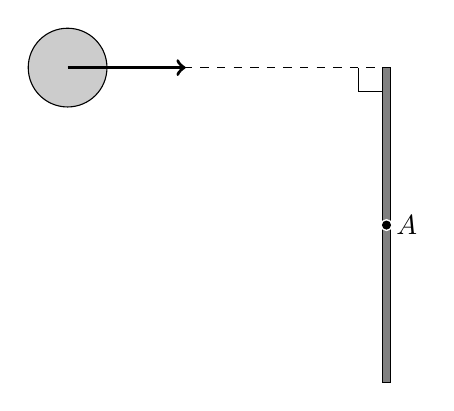
\begin{tikzpicture}
        %% ball of clay
        \node[draw,circle,minimum size=1cm,fill=white!80!black] (B) at (-4,0) {};
        \draw[dashed] (B.center) -- (0,0);
        \draw[very thick,->] (B.center) -- ++(0:1.5cm);
        %% thin rod
        \draw[fill=white!50!black] (0,0) rectangle (0.1,-4);
        \draw[fill=white,white] (0.05,-2) circle (0.07);
        \draw[fill] (0.05,-2) circle (0.05) node[anchor=west] {$A$};
        %% angle
        \draw (-0.3,0) -- (-0.3,-0.3) -- (0,-0.3);
    \end{tikzpicture}
    \end{center}
    The ball sticks to the rod. 
    After the collision, the angular momentum of the clay-rod system about $A$,
        the midpoint of the rod, is:
    \begin{multicols}{2}
    \begin{choices}
        \wrongchoice{$\left(m+\dfrac{M}{3}\right)\left(\dfrac{vL}{2}\right)$}
        \wrongchoice{$\left(m+\dfrac{M}{12}\right)\left(\dfrac{vL}{2}\right)$}
        \wrongchoice{$\left(m+\dfrac{M}{6}\right)\left(\dfrac{vL}{2}\right)$}
      \correctchoice{$\dfrac{mvL}{2}$}
        \wrongchoice{$mvL$}
    \end{choices}
    \end{multicols}
\end{question}
}

\element{serway-mc}{
\begin{question}{serway-ch11-q16}
    A particle of mass $m=\SI{0.10}{\kilo\gram}$ and speed $v_0=\SI{5.0}{\meter\per\second}$ collides and sticks to the end of a uniform solid cylinder of mass $M=\SI{1.0}{\kilo\gram}$ and radius $R=\SI{20}{\centi\meter}$.
    \begin{center}
    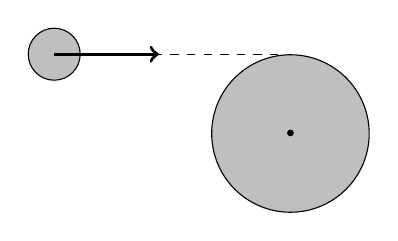
\begin{tikzpicture}
        \node[draw,circle,fill=white!75!black,minimum size=0.66cm,anchor=center] (A) at (-1,0) {};
        \node[draw,circle,fill=white!75!black,minimum size=2cm,anchor=north] (B) at (+2,0) {};
        \draw[dashed] (A.center) -- (B.north);
        \draw[very thick,->] (A.center) -- ++(0:1.33cm) node[pos=0.66,anchor=south] {};
        \draw[fill] (2,-1) circle (1pt);
    \end{tikzpicture}
    \end{center}
    If the cylinder is initially at rest and is pivoted about a frictionless axle through its center,
        what is the final angular velocity of the system after the collision?
    \begin{multicols}{2}
    \begin{choices}
        \wrongchoice{\SI{8.1}{\radian\per\second}}
        \wrongchoice{\SI{2.0}{\radian\per\second}}
        \wrongchoice{\SI{6.1}{\radian\per\second}}
      \correctchoice{\SI{4.2}{\radian\per\second}}
        \wrongchoice{\SI{10}{\radian\per\second}}
    \end{choices}
    \end{multicols}
\end{question}
}

\element{serway-mc}{
\begin{question}{serway-ch11-q17}
    A skater extends her arms horizontally,
        holding a \SI{5}{\kilo\gram} mass in each hand. 
    She is rotating about a vertical axis with an angular velocity of one revolution per second. 
    If she drops her hands to her sides,
        what will the final angular velocity be if her moment of inertia remains approximately constant at \SI{5}{\kilo\gram\meter\squared},
        and the distance of the masses from the axis changes from \SI{1.0}{\meter} to \SI{0.1}{\meter}?
    \begin{multicols}{3}
    \begin{choices}
         \wrongchoice{\SI{6}{\revolution\per\second}}
       \correctchoice{\SI{3}{\revolution\per\second}}
         \wrongchoice{\SI{9}{\revolution\per\second}}
         \wrongchoice{\SI{4}{\revolution\per\second}}
         \wrongchoice{\SI{7}{\revolution\per\second}}
    \end{choices}
    \end{multicols}
\end{question}
}

\element{serway-mc}{
\begin{question}{serway-ch11-q18}
    A merry-go-round of radius $R=\SI{2.0}{\meter}$ has a moment of inertia $I=\SI{250}{\kilo\gram\meter\squared}$,
        and is rotating at \SI{10}{\rotation\per\minute}. 
    A child whose mass is \SI{25}{\kilo\gram} jumps onto the edge of the merry-go-round, heading directly toward the center at \SI{6.0}{\meter\per\second}.
    The new angular speed (in rpm) of the merry-go-round is approximately:
    \begin{multicols}{2}
    \begin{choices}
        \wrongchoice{\SI{10}{\rotation\per\minute}}
        \wrongchoice{\SI{9.2}{\rotation\per\minute}}
        \wrongchoice{\SI{8.5}{\rotation\per\minute}}
      \correctchoice{\SI{7.1}{\rotation\per\minute}}
        \wrongchoice{\SI{6.4}{\rotation\per\minute}}
    \end{choices}
    \end{multicols}
\end{question}
}

\element{serway-mc}{
\begin{question}{serway-ch11-q19}
    A solid sphere (radius $R$, mass $M$) rolls without slipping down an incline as shown in the figure. 
    \begin{center}
    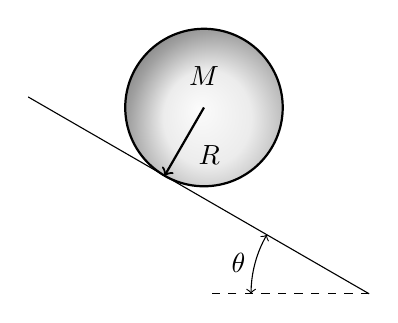
\begin{tikzpicture}
        %% Ground
        \draw[dashed] (0,0) -- (-2,0);
        \draw[<->] (-1.5,0) arc (180:150:1.5) node[anchor=east,pos=0.5] {$\theta$};
        %% Plane
        \draw (0,0) -- (150:5);
        %% Solid Sphere
        \draw[shading=ball,ball color=white!90!black,thick] (0,0) ++(150:3) ++(60:1) circle (1cm) node[anchor=south,yshift=1ex] {$M$};
        \draw[thick,<-] (0,0) ++(150:3) -- ++(60:1) node[pos=0.6,anchor=north west] {$R$};
    \end{tikzpicture}
    \end{center}
    The linear acceleration of its center of mass is:
    \begin{multicols}{3}
    \begin{choices}
      \correctchoice{$\dfrac{5g}{7}\sin\theta$}
        \wrongchoice{$\dfrac{3g}{5}\sin\theta$}
        \wrongchoice{$\dfrac{2g}{3}\sin\theta$}
        \wrongchoice{$\dfrac{g}{2}\sin\theta$}
        \wrongchoice{$\dfrac{4g}{5}\sin\theta$}
    \end{choices}
    \end{multicols}
\end{question}
}

\element{serway-mc}{
\begin{question}{serway-ch11-q20}
    A solid cylinder (radius $R$, mass $M$) rolls without slipping down an incline as shown in the figure. 
    \begin{center}
    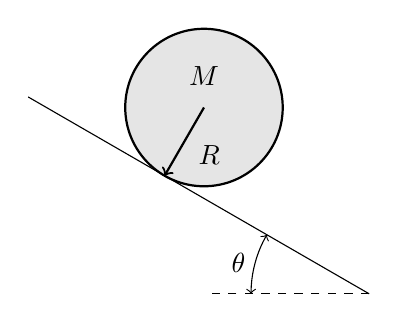
\begin{tikzpicture}
        %% Ground
        \draw[dashed] (0,0) -- (-2,0);
        \draw[<->] (-1.5,0) arc (180:150:1.5) node[anchor=east,pos=0.5] {$\theta$};
        %% Plane
        \draw (0,0) -- (150:5);
        %% Solid cylinder
        \draw[fill=white!90!black,thick] (0,0) ++(150:3) ++(60:1) circle (1cm) node[anchor=south,yshift=1ex] {$M$};
        \draw[thick,<-] (0,0) ++(150:3) -- ++(60:1) node[pos=0.6,anchor=north west] {$R$};
    \end{tikzpicture}
    \end{center}
    The linear acceleration of its center of mass is:
    \begin{multicols}{3}
    \begin{choices}
        \wrongchoice{$\dfrac{5g}{7}\sin\theta$}
        \wrongchoice{$\dfrac{1g}{2}\sin\theta$}
      \correctchoice{$\dfrac{2g}{3}\sin\theta$}
        \wrongchoice{$\dfrac{3g}{5}\sin\theta$}
        \wrongchoice{$\dfrac{4g}{5}\sin\theta$}
    \end{choices}
    \end{multicols}
\end{question}
}

\element{serway-mc}{
\begin{question}{serway-ch11-q21}
    A cylindrical shell (radius $R$, mass $M$) rolls without slipping down an incline as shown in the figure. 
    \begin{center}
    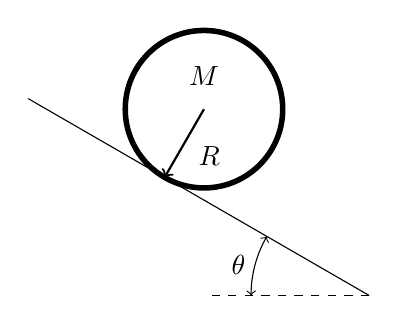
\begin{tikzpicture}
        %% Ground
        \draw[dashed] (0,0) -- (-2,0);
        \draw[<->] (-1.5,0) arc (180:150:1.5) node[anchor=east,pos=0.5] {$\theta$};
        %% Plane
        \draw (0,0) -- (150:5);
        %% Solid Sphere
        \draw[line width=2pt] (0,0) ++(150:3) ++(60:1) circle (1cm) node[anchor=south,yshift=1ex] {$M$};
        \draw[thick,<-] (0,0) ++(150:3) -- ++(60:1) node[pos=0.6,anchor=north west] {$R$};
    \end{tikzpicture}
    \end{center}
    The linear acceleration of its center of mass is:
    \begin{multicols}{3}
    \begin{choices}
        \wrongchoice{$\dfrac{5g}{7}\sin\theta$}
      \correctchoice{$\dfrac{g}{2}\sin\theta$}
        \wrongchoice{$\dfrac{3g}{5}\sin\theta$}
        \wrongchoice{$\dfrac{2g}{3}\sin\theta$}
        \wrongchoice{$\dfrac{4g}{5}\sin\theta$}
    \end{choices}
    \end{multicols}
\end{question}
}

\element{serway-mc}{
\begin{question}{serway-ch11-q22}
    A solid sphere, spherical shell,
        solid cylinder and a cylindrical shell all have the same mass $m$ and radius $R$. 
    If they are all released from rest at the same elevation and roll without slipping,
        which reaches the bottom of an inclined plane first?
    \begin{choices}
      \correctchoice{solid sphere}
        \wrongchoice{spherical shell}
        \wrongchoice{solid cylinder}
        \wrongchoice{cylindrical shell}
        \wrongchoice{all take the same time}
    \end{choices}
\end{question}
}

\element{serway-mc}{
\begin{question}{serway-ch11-q23}
    Stars originate as large bodies of slowly rotating gas. 
    Because of gravity,
        these clumps of gas slowly decrease in size. 
    The angular velocity of a star increases as it shrinks because of:
    \begin{choices}
      \correctchoice{conservation of angular momentum}
        \wrongchoice{conservation of linear momentum}
        \wrongchoice{conservation of energy}
        \wrongchoice{the law of universal gravitation}
        \wrongchoice{conservation of mass}
    \end{choices}
\end{question}
}

\element{serway-mc}{
\begin{question}{serway-ch11-q24}
    Five objects of mass $m$ move at velocity $v$ at a distance $r$ from an axis of rotation perpendicular to the page through point $A$,
        as shown below. 
    The one that has zero angular momentum about that axis is:
    \begin{multicols}{2}
    \begin{choices}
        \AMCboxDimensions{down=-1.5cm}
        \wrongchoice{
            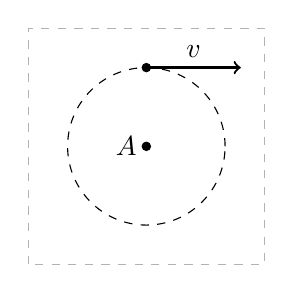
\begin{tikzpicture}
                \draw[dashed,white!70!black] (-1.5,-1.5) rectangle (1.5,1.5);
                \draw[dashed] (0,0) circle (1cm);
                \draw[fill] (0,0) circle (1.5pt) node[anchor=east] {$A$};
                \draw[fill] (0,1) circle (1.5pt);
                \draw[thick,->] (0,1) -- ++(0:1.2) node[pos=0.5,anchor=south] {$v$};
            \end{tikzpicture}
        }
        \wrongchoice{
            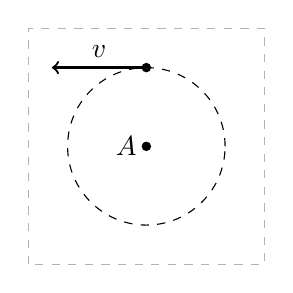
\begin{tikzpicture}
                \draw[dashed,white!70!black] (-1.5,-1.5) rectangle (1.5,1.5);
                \draw[dashed] (0,0) circle (1cm);
                \draw[fill] (0,0) circle (1.5pt) node[anchor=east] {$A$};
                \draw[fill] (0,1) circle (1.5pt);
                \draw[thick,->] (0,1) -- ++(180:1.2) node[pos=0.5,anchor=south] {$v$};
            \end{tikzpicture}
        }
        \wrongchoice{
            \begin{tikzpicture}
                \draw[dashed,white!70!black] (-1,-1) rectangle (2,2);
                \draw[fill] (0,0) circle (1.5pt) node[anchor=east] {$A$};
                \draw[fill] (0,1) circle (1.5pt);
                \draw[thick,->] (0,1) -- ++(0:1.2) node[pos=0.5,anchor=south] {$v$};
            \end{tikzpicture}
        }
        %% ANS is D
        \correctchoice{
            \begin{tikzpicture}
                \draw[dashed,white!70!black] (-1,-1) rectangle (2,2);
                \draw[fill] (0,0) circle (1.5pt) node[anchor=east] {$A$};
                \draw[fill] (45:1) circle (1.5pt);
                \draw[thick,->] (45:1) -- ++(45:1.2) node[pos=0.5,anchor=south] {$v$};
            \end{tikzpicture}
        }
        \wrongchoice{
            \begin{tikzpicture}
                \draw[dashed,white!70!black] (-1,-1) rectangle (2,2);
                \draw[fill] (0,0) circle (1.5pt) node[anchor=east] {$A$};
                \draw[fill] (30:1) circle (1.5pt);
                \draw[thick,->] (30:1) -- ++(45:1.2) node[pos=0.5,anchor=south] {$v$};
            \end{tikzpicture}
        }
    \end{choices}
    \end{multicols}
\end{question}
}

\element{serway-mc}{
\begin{question}{serway-ch11-q25}
    The object shown below has mass $m$ and velocity $v$. 
    \begin{center}
    \begin{tikzpicture}
        \draw[dashed] (-2,0) -- (2,0);
        \draw[fill] (0,-1) circle (1.5pt) node[anchor=west] {$O$};
        \draw[thick,->] (2,0) -- ++(0:1cm);
    \end{tikzpicture}
    \end{center}
    The direction of its angular momentum vector with respect to an axis perpendicular to the page through point $O$ is:
    \begin{choices}
        \wrongchoice{downwards.}
        \wrongchoice{to the right.}
      \correctchoice{into the page.}
        \wrongchoice{up out of the page.}
        \wrongchoice{counterclockwise.}
    \end{choices}
\end{question}
}

\element{serway-mc}{
\begin{question}{serway-ch11-q26}
    Two objects of mass $m_1=2m$ and $m_2=m$ move around a rotation axis $O$ in parallel circles of radii $r_1=r$ and $r_2=2r$ with equal tangential speeds. 
    \begin{center}
    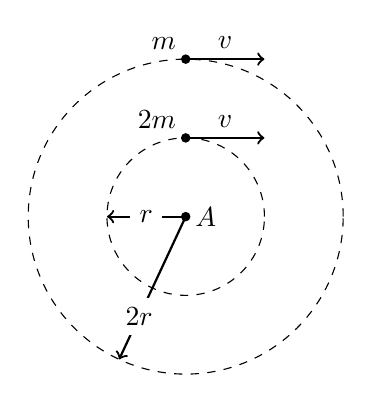
\begin{tikzpicture}
        %% Labels
        \draw[fill] (0,0) circle (1.5pt) node[anchor=west] {$A$};
        \draw[fill] (0,1) circle (1.5pt) node[anchor=south east] {$2m$};
        \draw[thick,->] (0,1) -- ++(0:1cm) node[anchor=south,pos=0.5] {$v$};
        \draw[fill] (0,2) circle (1.5pt) node[anchor=south east] {$m$};
        \draw[thick,->] (0,2) -- ++(0:1cm) node[anchor=south,pos=0.5] {$v$};
        %% Radii
        \draw[thick,->] (0,0) -- (180:1) node[pos=0.5,fill=white,anchor=center] {$r$};
        \draw[thick,->] (0,0) -- (245:2) node[pos=0.7,fill=white,anchor=center] {$2r$};
        %% Circles
        \draw[dashed] (0,0) circle (1cm);
        \draw[dashed] (0,0) circle (2cm);
    \end{tikzpicture}
    \end{center}
    As they rotate,
        forces of equal magnitude are applied opposite to their velocities to stop them. Which statement is correct?
    \begin{choices}
        \wrongchoice{$m_2$ will stop first because it has the larger initial angular velocity.}
        \wrongchoice{$m_1$ will stop first because it has the smaller radius.}
      \correctchoice{$m_2$ will stop first because the torque on it is greater.}
        \wrongchoice{$m_1$ will stop first because it has the smaller moment of inertia.}
        \wrongchoice{Both objects will stop at the same time because the angular accelerations are equal.}
    \end{choices}
\end{question}
}

\element{serway-mc}{
\begin{question}{serway-ch11-q27}
    A torque can be exerted on a body with a fixed axis of rotation:
    \begin{choices}
        \wrongchoice{only by a centripetal force.}
        \wrongchoice{only by a force directed radially outwards.}
        \wrongchoice{only by a tangential force.}
        \wrongchoice{only by a force with a component directed radially outwards.}
      \correctchoice{by any force perpendicular to but not pointing directly toward or away from the axis of rotation.}
    \end{choices}
\end{question}
}

\element{serway-mc}{
\begin{question}{serway-ch11-q28}
    Five identical cylinders are each acted on by forces of equal magnitude. 
    Which force exerts the biggest torque?
    \begin{multicols}{2}
    \begin{choices}
        \AMCboxDimensions{down=-1.25cm}
        %% ANS is A
        \correctchoice{
            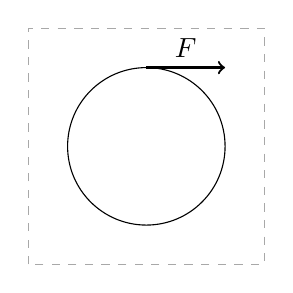
\begin{tikzpicture}
                \draw[dashed,white!66!black] (-1.5,-1.5) rectangle (1.5,1.5);
                \draw (0,0) circle (1cm);
                \draw[thick,->] (0,1) -- ++(0:1cm) node[anchor=south,pos=0.5] {$F$};
            \end{tikzpicture}
        }
        \wrongchoice{
            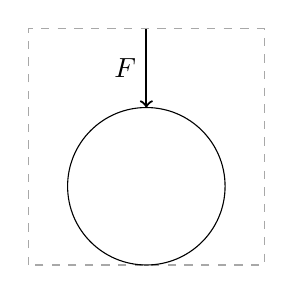
\begin{tikzpicture}
                \draw[dashed,white!66!black] (-1.5,-1.0) rectangle (1.5,2.0);
                \draw (0,0) circle (1cm);
                \draw[thick,<-] (0,1) -- ++(90:1cm) node[anchor=east,pos=0.5] {$F$};
            \end{tikzpicture}
        }
        \wrongchoice{
            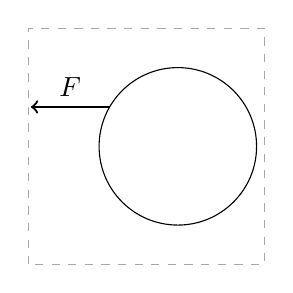
\begin{tikzpicture}
                \draw[dashed,white!66!black] (-1.9,-1.5) rectangle (1.1,1.5);
                \draw (0,0) circle (1cm);
                \draw[thick,->] (150:1) -- ++(180:1cm) node[anchor=south,pos=0.5] {$F$};
            \end{tikzpicture}
        }
        \wrongchoice{
            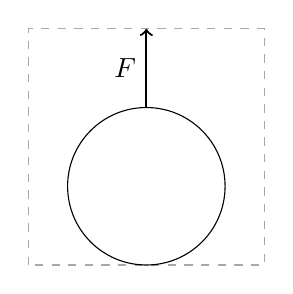
\begin{tikzpicture}
                \draw[dashed,white!66!black] (-1.5,-1.0) rectangle (1.5,2.0);
                \draw (0,0) circle (1cm);
                \draw[thick,->] (90:1) -- ++(90:1cm) node[anchor=east,pos=0.5] {$F$};
            \end{tikzpicture}
        }
        \wrongchoice{
            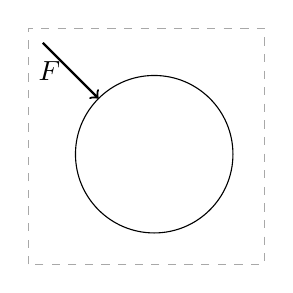
\begin{tikzpicture}
                \draw[dashed,white!66!black] (-1.6,-1.4) rectangle (1.4,1.6);
                \draw (0,0) circle (1cm);
                \draw[thick,<-] (135:1) -- ++(135:1cm) node[anchor=east,pos=0.5] {$F$};
            \end{tikzpicture}
        }
    \end{choices}
    \end{multicols}
\end{question}
}

\element{serway-mc}{
\begin{question}{serway-ch11-q29}
    The diagram below shows five cylinders,
        each cylinder rotating with constant angular velocity about its central axis. 
    The magnitude of the tangential velocity of one point of each cylinder is shown,
        along with each cylinder's radius and mass. 
    Which cylinder has the largest angular momentum?
    \begin{multicols}{2}
    \begin{choices}
        \AMCboxDimensions{down=-1.5cm}
        \wrongchoice{
            \begin{tikzpicture}[scale=0.75]
                \draw[dashed,white!66!black] (-2.1,-2.3) rectangle (2.1,2.7);
                \draw (0,0) circle (1cm);
                \draw[thick,->] (0,1) -- ++(180:1cm) node[anchor=south,pos=0.5] {$v=\SI{2}{\meter\per\second}$};
                \node[anchor=north,text centered,text width=5em] at (0,-1) {$r=\SI{2}{\meter}$ \\ $M=\SI{20}{\kilo\gram}$};
            \end{tikzpicture}
        }
        \wrongchoice{
            \begin{tikzpicture}[scale=0.75]
                \draw[dashed,white!66!black] (-2.1,-2.3) rectangle (2.1,2.7);
                \draw (0,0) circle (1cm);
                \draw[thick,->] (0,1) -- ++(180:2cm) node[anchor=south,pos=0.5] {$v=\SI{4}{\meter\per\second}$};
                \node[anchor=north,text centered,text width=5em] at (0,-1) {$r=\SI{2}{\meter}$ \\ $M=\SI{20}{\kilo\gram}$};
            \end{tikzpicture}
        }
        \wrongchoice{
            \begin{tikzpicture}[scale=0.75]
                \draw[dashed,white!66!black] (-2.1,-2.3) rectangle (2.1,2.7);
                \draw (0,0) circle (1cm);
                \draw[thick,->] (0,1) -- ++(180:1cm) node[anchor=south,pos=0.5] {$v=\SI{2}{\meter\per\second}$};
                \node[anchor=north,text centered,text width=5em] at (0,-1) {$r=\SI{2}{\meter}$ \\ $M=\SI{20}{\kilo\gram}$};
            \end{tikzpicture}
        }
        %% big circle
        \wrongchoice{
            \begin{tikzpicture}[scale=0.75]
                \draw[dashed,white!66!black] (-2.1,-2.3) rectangle (2.1,2.7);
                \draw (0,0) circle (2cm);
                \draw[thick,->] (0,2) -- ++(180:1cm) node[anchor=south,pos=0.5] {$v=\SI{2}{\meter\per\second}$};
                \node[anchor=north,text centered,text width=5em] at (0,0) {$r=\SI{4}{\meter}$ \\ $M=\SI{10}{\kilo\gram}$};
            \end{tikzpicture}
        }
        %% ANS is E
        \correctchoice{
            \begin{tikzpicture}[scale=0.75]
                \draw[dashed,white!66!black] (-2.1,-2.3) rectangle (2.1,2.7);
                \draw (0,0) circle (1cm);
                \draw[thick,->] (0,1) -- ++(180:2cm) node[anchor=south,pos=0.5] {$v=\SI{4}{\meter\per\second}$};
                \node[anchor=north,text centered,text width=5em] at (0,-1) {$r=\SI{2}{\meter}$ \\ $M=\SI{20}{\kilo\gram}$};
            \end{tikzpicture}
        }
    \end{choices}
    \end{multicols}
\end{question}
}

\element{serway-mc}{
\begin{question}{serway-ch11-q30}
    The diagram below shows five thin cylindrical shells,
        each shell rotating with constant angular velocity about its central axis. 
    The magnitude of the tangential velocity of one point of each cylinder is shown,
        along with each cylinder’s radius and mass. 
    Which cylindrical shell has the largest angular momentum?
    \begin{multicols}{2}
    \begin{choices}
        \AMCboxDimensions{down=-1.5cm}
        \wrongchoice{
            \begin{tikzpicture}[scale=0.75]
                \draw[dashed,white!66!black] (-2.1,-2.3) rectangle (2.1,2.7);
                \draw[fill=white!60!black] (0,0) circle (1cm);
                \draw[fill=white] (0,0) circle (0.8cm);
                \draw[thick,->] (0,1) -- ++(180:1cm) node[anchor=south,pos=0.5] {$v=\SI{2}{\meter\per\second}$};
                \node[anchor=north,text centered,text width=5em] at (0,-1) {$r=\SI{2}{\meter}$ \\ $M=\SI{20}{\kilo\gram}$};
            \end{tikzpicture}
        }
        \wrongchoice{
            \begin{tikzpicture}[scale=0.75]
                \draw[dashed,white!66!black] (-2.1,-2.3) rectangle (2.1,2.7);
                \draw[fill=white!60!black] (0,0) circle (1cm);
                \draw[fill=white] (0,0) circle (0.8cm);
                \draw[thick,->] (0,1) -- ++(180:2cm) node[anchor=south,pos=0.5] {$v=\SI{4}{\meter\per\second}$};
                \node[anchor=north,text centered,text width=5em] at (0,-1) {$r=\SI{2}{\meter}$ \\ $M=\SI{20}{\kilo\gram}$};
            \end{tikzpicture}
        }
        \wrongchoice{
            \begin{tikzpicture}[scale=0.75]
                \draw[dashed,white!66!black] (-2.1,-2.3) rectangle (2.1,2.7);
                \draw[fill=white!60!black] (0,0) circle (1cm);
                \draw[fill=white] (0,0) circle (0.8cm);
                \draw[thick,->] (0,1) -- ++(180:1cm) node[anchor=south,pos=0.5] {$v=\SI{2}{\meter\per\second}$};
                \node[anchor=north,text centered,text width=5em] at (0,-1) {$r=\SI{2}{\meter}$ \\ $M=\SI{20}{\kilo\gram}$};
            \end{tikzpicture}
        }
        %% big circle
        \wrongchoice{
            \begin{tikzpicture}[scale=0.75]
                \draw[dashed,white!66!black] (-2.1,-2.3) rectangle (2.1,2.7);
                \draw[fill=white!60!black] (0,0) circle (2cm);
                \draw[fill=white] (0,0) circle (1.8cm);
                \draw[thick,->] (0,2) -- ++(180:1cm) node[anchor=south,pos=0.5] {$v=\SI{2}{\meter\per\second}$};
                \node[anchor=north,text centered,text width=5em] at (0,0) {$r=\SI{4}{\meter}$ \\ $M=\SI{10}{\kilo\gram}$};
            \end{tikzpicture}
        }
        %% ANS is E
        \correctchoice{
            \begin{tikzpicture}[scale=0.75]
                \draw[dashed,white!66!black] (-2.1,-2.3) rectangle (2.1,2.7);
                \draw[fill=white!60!black] (0,0) circle (1cm);
                \draw[fill=white] (0,0) circle (0.8cm);
                \draw[thick,->] (0,1) -- ++(180:2cm) node[anchor=south,pos=0.5] {$v=\SI{4}{\meter\per\second}$};
                \node[anchor=north,text centered,text width=5em] at (0,-1) {$r=\SI{2}{\meter}$ \\ $M=\SI{20}{\kilo\gram}$};
            \end{tikzpicture}
        }
    \end{choices}
    \end{multicols}
\end{question}
}

\element{serway-mc}{
\begin{question}{serway-ch11-q31}
    The diagram below shows five \SI{20}{\kilo\gram} rods of the same \SI{2.0}{\meter} length free to rotate about axes through the rods,
        as indicated.
    Which rod experiences the greatest gravitational torque?
    \begin{multicols}{2}
    \begin{choices}
        \AMCboxDimensions{down=-0.6cm}
        \wrongchoice{
            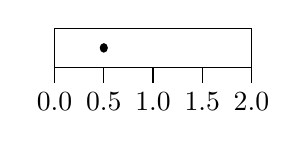
\begin{tikzpicture}[xscale=1.25]
                \draw (0,0) rectangle (2,0.5);
                \draw[fill] (0.5,0.25) circle (1pt and 1.5pt);
                \draw (0.0,0) -- (0.0,-0.2) node[anchor=north] {$0.0$};
                \draw (0.5,0) -- (0.5,-0.2) node[anchor=north] {$0.5$};
                \draw (1.0,0) -- (1.0,-0.2) node[anchor=north] {$1.0$};
                \draw (1.5,0) -- (1.5,-0.2) node[anchor=north] {$1.5$};
                \draw (2.0,0) -- (2.0,-0.2) node[anchor=north] {$2.0$};
            \end{tikzpicture}
        }
        \wrongchoice{
            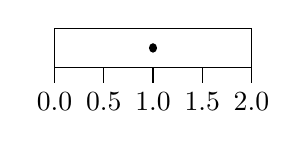
\begin{tikzpicture}[xscale=1.25]
                \draw (0,0) rectangle (2,0.5);
                \draw[fill] (1.0,0.25) circle (1pt and 1.5pt);
                \draw (0.0,0) -- (0.0,-0.2) node[anchor=north] {$0.0$};
                \draw (0.5,0) -- (0.5,-0.2) node[anchor=north] {$0.5$};
                \draw (1.0,0) -- (1.0,-0.2) node[anchor=north] {$1.0$};
                \draw (1.5,0) -- (1.5,-0.2) node[anchor=north] {$1.5$};
                \draw (2.0,0) -- (2.0,-0.2) node[anchor=north] {$2.0$};
            \end{tikzpicture}
        }
        \wrongchoice{
            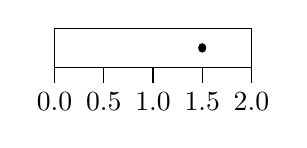
\begin{tikzpicture}[xscale=1.25]
                \draw (0,0) rectangle (2,0.5);
                \draw[fill] (1.5,0.25) circle (1pt and 1.5pt);
                \draw (0.0,0) -- (0.0,-0.2) node[anchor=north] {$0.0$};
                \draw (0.5,0) -- (0.5,-0.2) node[anchor=north] {$0.5$};
                \draw (1.0,0) -- (1.0,-0.2) node[anchor=north] {$1.0$};
                \draw (1.5,0) -- (1.5,-0.2) node[anchor=north] {$1.5$};
                \draw (2.0,0) -- (2.0,-0.2) node[anchor=north] {$2.0$};
            \end{tikzpicture}
        }
        \wrongchoice{
            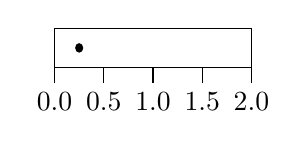
\begin{tikzpicture}[xscale=1.25]
                \draw (0,0) rectangle (2,0.5);
                \draw[fill] (0.25,0.25) circle (1pt and 1.5pt);
                \draw (0.0,0) -- (0.0,-0.2) node[anchor=north] {$0.0$};
                \draw (0.5,0) -- (0.5,-0.2) node[anchor=north] {$0.5$};
                \draw (1.0,0) -- (1.0,-0.2) node[anchor=north] {$1.0$};
                \draw (1.5,0) -- (1.5,-0.2) node[anchor=north] {$1.5$};
                \draw (2.0,0) -- (2.0,-0.2) node[anchor=north] {$2.0$};
            \end{tikzpicture}
        }
        %% ANS is E
        \correctchoice{
            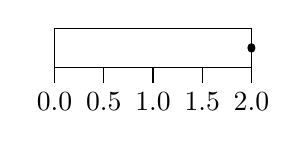
\begin{tikzpicture}[xscale=1.25]
                \draw (0,0) rectangle (2,0.5);
                \draw[fill] (2.0,0.25) circle (1pt and 1.5pt);
                \draw (0.0,0) -- (0.0,-0.2) node[anchor=north] {$0.0$};
                \draw (0.5,0) -- (0.5,-0.2) node[anchor=north] {$0.5$};
                \draw (1.0,0) -- (1.0,-0.2) node[anchor=north] {$1.0$};
                \draw (1.5,0) -- (1.5,-0.2) node[anchor=north] {$1.5$};
                \draw (2.0,0) -- (2.0,-0.2) node[anchor=north] {$2.0$};
            \end{tikzpicture}
        }
    \end{choices}
    \end{multicols}
\end{question}
}

\element{serway-mc}{
\begin{question}{serway-ch11-q32}
    A force $\vec{\mathbf{F}}$ is applied to a cylindrical roll of paper of radius $R$ and mass $M$ by pulling on the paper as shown. 
    \begin{center}
    \begin{tikzpicture}
        %% Floor
        \draw (-3,0) -- (3,0);
        \node[anchor=north,fill,pattern=north east lines,minimum width=6cm, minimum height=0.05cm] at (0,0) {};
        %% Cylinder
        \draw[thick,fill=white!90!black] (0,1) circle (1cm);
        \draw[ultra thick,->] (0,2) -- (2,2) node[anchor=south,pos=0.5] {$F$};
    \end{tikzpicture}
    \end{center}
    The acceleration of the center of mass of the roll of paper
        (when it rolls without slipping) is:
    \begin{multicols}{3}
    \begin{choices}
        \wrongchoice{$\dfrac{F}{2M}$}
        \wrongchoice{$\dfrac{F}{M}$}
        \wrongchoice{$\dfrac{3F}{2M}$}
      \correctchoice{$\dfrac{4F}{3M}$}
        \wrongchoice{$\dfrac{2F}{M}$}
    \end{choices}
    \end{multicols}
\end{question}
}

%\element{serway-mc}{
%\begin{question}{serway-ch11-q33}
%    A \SI{0.5}{\kilo\gram} fish, hooked as shown below,
%        starts to swim away at a speed of \SI{3}{\meter\per\second}.
%    \begin{center}
%    \begin{tikzpicture}
%        %% NOTE: TODO: draw tikz
%        %% Fish
%        \draw[fill] (0,0) circle (3pt) node[anchor=north west] {fish};
%        \draw[very thick,->] (0,0) -- (1,0) node[anchor=west] {$v=\SI{3}{\meter\per\second}$};
%        %% 10 m
%    \end{tikzpicture}
%    \end{center}
%    The angular momentum of the fish relative to the
%        hand holding the fishing rod is:
%    \begin{multicols}{2}
%    \begin{choices}
%      \correctchoice{\SI{3}{\kilo\gram\meter\squared\per\second}}
%        \wrongchoice{\SI{6}{\kilo\gram\meter\squared\per\second}}
%        \wrongchoice{\SI{17}{\kilo\gram\meter\squared\per\second}}
%        \wrongchoice{\SI{30}{\kilo\gram\meter\squared\per\second}}
%        \wrongchoice{\SI{60}{\kilo\gram\meter\squared\per\second}}
%    \end{choices}
%    \end{multicols}
%\end{question}
%}

\element{serway-mc}{
\begin{question}{serway-ch11-q34}
    The \SI{1560}{\kilo\gram} steel door to a bank vault is \SI{2.00}{\meter} high,
        \SI{1.00}{\meter} wide and \SI{10}{\centi\meter} thick.
    One hinge is \SI{60.0}{\centi\meter} down from the top on the left side of the door.
    The other hinge is \SI{30.0}{\centi\meter} up from the bottom.
    What horizontal force, in what direction, does the door exert on the upper hinge.
    \begin{multicols}{2}
    \begin{choices}
      \correctchoice{\SI{6950}{\newton}, left}
        \wrongchoice{\SI{6950}{\newton}, right}
        \wrongchoice{\SI{7640}{\newton}, left}
        \wrongchoice{\SI{7640}{\newton}, right}
        \wrongchoice{\SI{15 300}{\newton}, left}
    \end{choices}
    \end{multicols}
\end{question}
}

\element{serway-mc}{
\begin{question}{serway-ch11-q35}
    The \SI{1560}{\kilo\gram} solid steel door to a bank vault is \SI{2.00}{\meter} high,
        \SI{1.00}{\meter} wide and \SI{10}{\centi\meter} thick. 
    One hinge is \SI{60.0}{\centi\meter} down from the top on the left hand side of the door.
    The other hinge is \SI{30.0}{\centi\meter} up from the bottom. 
    What horizontal force, in what direction,
        does the door exert on the upper hinge?
    \begin{multicols}{2}
    \begin{choices}
        \wrongchoice{\SI{6950}{\newton}, left}
      \correctchoice{\SI{6950}{\newton}, right}
        \wrongchoice{\SI{7640}{\newton}, left}
        \wrongchoice{\SI{7640}{\newton}, right}
        \wrongchoice{\SI{15,300}{\newton}, left}
    \end{choices}
    \end{multicols}
\end{question}
}

\element{serway-mc}{
\begin{question}{serway-ch11-q36}
    The free body diagram below represents a \SI{1500}{\kilo\gram} car sitting on a \SI{3000}{\kilo\gram} bridge supported at its far ends.
    The car's position is three quarters of the length $L$ from the left end of the bridge. 
    Identify the error in the equation below:
    \begin{align*}
        -\left(\dfrac{L}{2}\right) F_{Earth on bridge}
        -&\left(\dfrac{3L}{4}\right) F_{Earth on car} \\
         &- LF_1 + LF_2 = 0
    \end{align*}
    \begin{center}
    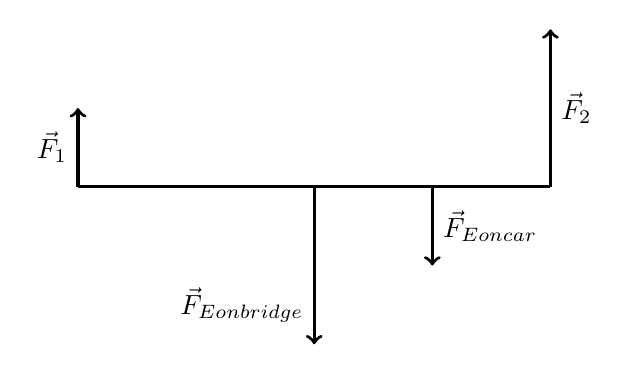
\begin{tikzpicture}
        \draw[very thick] (-3,0) -- (3,0);
        \draw[very thick,->] (-3,0) -- (-3,1) node[pos=0.5,anchor=east] {$\vec{F}_1$};
        \draw[very thick,->] (0,0) -- (0,-2) node[pos=0.75,anchor=east] {$\vec{F}_{\text{E on bridge}}$};
        \draw[very thick,->] (1.5,0) -- (1.5,-1) node[pos=0.5,anchor=west] {$\vec{F}_{\text{E on car}}$};
        \draw[very thick,->] (3,0) -- (3,2) node[pos=0.5,anchor=west] {$\vec{F}_2$};
    \end{tikzpicture}
    \end{center}
    \begin{choices}
        \wrongchoice{$\vec{\mathbf{F}}_1$ never produces a torque on the bridge no matter where the axis of rotation is placed.}
        \wrongchoice{$\vec{\mathbf{F}}_2$ never produces a torque on the bridge no matter where the axis of rotation is placed.}
        \wrongchoice{Torques have been taken about two axes and summed.}
      \correctchoice{Because the perpendicular distance to $\vec{\mathbf{F}}_1$ from the left end of the bridge is 0, $LF_1$ should be 0.}
        \wrongchoice{Because the perpendicular distance to $\vec{\mathbf{F}}_2$ from the right end of the bridge is 0, $LF_2$ should be 0.}
    \end{choices}
\end{question}
}

\newcommand{\serwayChElevenQThirtySeven}{
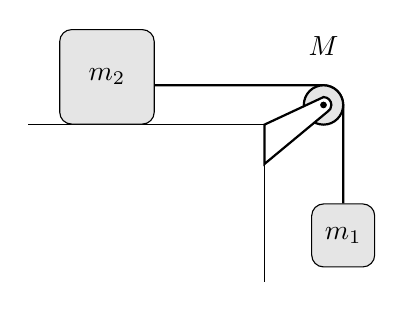
\begin{tikzpicture}
    %% Floor
    \draw (-3,0) -- (0,0) -- (0,-2);
    %% Mass
    \node[draw,fill=white!90!black,rectangle,rounded corners=1ex,minimum size=1.2cm,anchor=south] (A) at (-2,0) {$m_2$};
    \node[draw,fill=white!90!black,rectangle,rounded corners=1ex,minimum size=0.8cm,anchor=north] (B) at (1,-1) {$m_1$};
    %% Labels
    %\draw[thick,->] (-2,1.5) -- ++ (0:1) node[pos=0.5,anchor=south] {$a$};
    \node[anchor=south] at (0.75,0.75) {$M$};
    %% Rope and Pully
    \draw[thick] (A.south east) ++(90:0.5) -- (0.75,0.5) arc(90:0:0.25) -- (B.north);
    \draw[thick,fill=white!90!black] (0.75,0.25) circle (0.25); 
    \draw[thick,fill=white] (0,0) -- (0.75,0.35) arc (90:-60:0.1) -- (0,-0.5) -- cycle;
    \draw[fill] (0.75,0.25) circle (1pt);
\end{tikzpicture}
}

\element{serway-mc}{
\begin{question}{serway-ch11-q37}
    Two blocks of masses $m_1$ and $m_2$ are connected by a light cord that passes over a pulley of mass $M$,
        as shown.
    Block $m_2$ slides on a frictionless horizontal surface.
    The blocks and pulley are initially at rest. 
    When $m_1$ is released,
        the blocks accelerate and the pulley rotates. 
    \begin{center}
        \serwayChElevenQThirtySeven
    \end{center}
    The total angular momentum of the system of the two blocks and the pulley relative to the axis of rotation of the pulley is:
    \begin{choices}
        \wrongchoice{the same at all times.}
        \wrongchoice{proportional to $l_1$, the length of string from the pulley to $m_1$.}
        \wrongchoice{proportional to $l_2$, the length of string from the pulley to $m_2$.}
        \wrongchoice{conserved because the Earth doesn't move.}
      \correctchoice{proportional to the velocity of the blocks.}
    \end{choices}
\end{question}
}

\element{serway-mc}{
\begin{questionmult}{serway-ch11-q38}
    Two blocks of masses $m_1$ and $m_2$ are connected by a light cord that passes over a pulley of mass $M$,
        as shown. 
    Block $m_2$ slides on a frictionless horizontal surface.
    The blocks and pulley are initially at rest. 
    When $m_1$ is released,
        the blocks accelerate and the pulley rotates. 
    \begin{center}
        \serwayChElevenQThirtySeven
    \end{center}
    The total angular momentum of the system of the two blocks and the pulley relative to the axis of rotation of the pulley is:
    \begin{choices}
      \correctchoice{proportional to the radius of the pulley.}
      \correctchoice{proportional to the velocity of the blocks.}
        \wrongchoice{proportional to the length of the string.}
        %\wrongchoice{to all of the above.}
        %\correctchoice{only to (a) and (b) above.}
    \end{choices}
\end{questionmult}
}

\element{serway-mc}{
\begin{question}{serway-ch11-q39}
    When an object is effectively isolated from external torques,
        like an ice skater twirling on the tip of one skate,
        the angular momentum of the object:
    \begin{choices}
        \wrongchoice{can be increased by shifting mass out away from the axis of rotation.}
        \wrongchoice{can be decreased by shifting mass out away from the axis of rotation.}
        \wrongchoice{can be increased by shifting mass in toward the axis of rotation.}
        \wrongchoice{can be decreased by shifting mass in toward the axis of rotation.}
      \correctchoice{cannot be changed except by friction at the point of contact.}
    \end{choices}
\end{question}
}

\element{serway-mc}{
\begin{questionmult}{serway-ch11-q40}
    A hockey puck traveling at speed $v$ on essentially frictionless ice collides elastically with one end of a straight stick lying flat on the ice. 
    In this collision:
    \begin{choices}
      \correctchoice{momentum is conserved.}
      \correctchoice{angular momentum is conserved.}
      \correctchoice{mechanical energy is conserved.}
        %\correctchoice{all of the above are conserved.}
        %\wrongchoice{only momentum and angular momentum are conserved.}
    \end{choices}
\end{questionmult}
}

\element{serway-mc}{
\begin{questionmult}{serway-ch11-q41}
    A hockey puck traveling at speed $v$ on essentially frictionless ice collides with one end of a straight stick lying flat on the ice and sticks to that end.
    In this collision:
    \begin{choices}
      \correctchoice{momentum is conserved.}
      \correctchoice{angular momentum is conserved.}
        \wrongchoice{mechanical energy is conserved.}
        %\wrongchoice{all of the above are conserved.}
        %\wrongchoice{only momentum and angular momentum are conserved.}
    \end{choices}
\end{questionmult}
}

\element{serway-mc}{
\begin{question}{serway-ch11-q42}
    A space station out beyond the solar system is rotating with constant angular velocity. 
    A spaceship heading into the station along a diameter of the station,
        uses its rockets to brake, and then docks inside the station. 
    When the spaceship docks,
        the angular momentum of the system consisting of the station and ship:
    \begin{choices}
        \wrongchoice{is less than the original angular momentum of the station.}
      \correctchoice{is the same as the original angular momentum of the station.}
        \wrongchoice{is greater than the original angular momentum of the station.}
        \wrongchoice{is less than the original angular momentum of the station, but the angular velocity increases.}
        \wrongchoice{is greater than the original angular momentum of the station, but the angular velocity decreases.}
    \end{choices}
\end{question}
}


\endinput


